\chapter{Υπόβαθρο} \label{chapter:gr-background}

Σε αυτό το κεφάλαιο παραθέτουμε το απαραίτητο θεωρητικό υπόβαθρο για την
κατανόηση των κεντρικών ιδεών της διπλωματικής εργασίας.

\section{Η Εξέλιξη της Αρχιτεκτονικής των Εφαρμογών}

Η δημοτικότητα των μικροϋπηρεσιών και του containerization έχει εκραγεί τα
τελευταία χρόνια. Η ανάγκη για κλιμακούμενες εφαρμογές που αναπτύσσονται εύκολα,
έχει οδηγήσει στην εγκατάλειψη των μονολιθικών αρχιτεκτονικών, όπου όλες οι
διαδικασίες είναι στενά συνδεδεμένες και εκτελούνται ως μια ενιαία υπηρεσία,
προς όφελος των μικροϋπηρεσιών. Οι μικροϋπηρεσίες είναι μια αρχιτεκτονική και
οργανωτική προσέγγιση στην ανάπτυξη λογισμικού, όπου το λογισμικό αποτελείται
από μικρές ανεξάρτητες υπηρεσίες που επικοινωνούν μέσω καλά ορισμένων APIs.

Η τρέχουσα τάση της βιομηχανίας αναφορικά με τις μικροϋπηρεσίες είναι η χρήση
του containerization για την παροχή μικρότερων, ενιαίων λειτουργικών μονάδων, οι
οποίες συνεργάζονται μεταξύ τους για τη δημιουργία ευέλικτων επεκτάσιμων
εφαρμογών. Το containerization είναι μια μορφή εικονικοποίησης όπου οι εφαρμογές
εκτελούνται σε απομονωμένους χώρους χρηστών, που ονομάζονται container, ενώ
χρησιμοποιούν το ίδιο κοινόχρηστο λειτουργικό σύστημα. Ένα container είναι
ουσιαστικά ένα πλήρες συσκευασμένο και φορητό υπολογιστικό περιβάλλον. Όλα όσα
χρειάζεται μια εφαρμογή για να εκτελεστεί --ο δυαδικός κώδικας, βιβλιοθήκες,
αρχεία ρυθμίσεων και εξαρτήσεις-- είναι ενσωματωμένα και απομονωμένα στο
container.

Η εκτεταμένη χρήση των containers, έχει οδηγήσει στην ανάγκη αυτοματοποίησης της
ανάπτυξης και της διαχείρισης τους. Η ενορχήστρωση containers είναι η
αυτοματοποίηση της προσπάθειας που απαιτείται για την εκτέλεση φορτίων εργασίας
σε container και υπηρεσιών. Αυτό περιλαμβάνει ένα ευρύ φάσμα ενεργειών που
χρειάζονται οι ομάδες λογισμικού για να διαχειριστούν τον κύκλο ζωής ενός
container, συμπεριλαμβανομένης της παροχής, της ανάπτυξης, της κλιμάκωσης, της
δικτύωσης, της εξισορρόπησης φορτίου κ.λπ.

Μεταξύ των διαφόρων ενορχηστρωτών containers, ο Kubernetes είναι η πιο δημοφιλής
λύση και πλέον αποτελεί το βιομηχανικό πρότυπο. Έχοντας αρχικά ξεκινήσει από την
Google, ο Kubernetes είναι μια φορητή, επεκτάσιμη, ανοιχτού κώδικα πλατφόρμα για
τη διαχείριση των containerized φόρτων εργασίας και υπηρεσιών, που διευκολύνει
τόσο τη δηλωτική παραμετροποίησή τους, όσο και την αυτοματοποίηση των
διαδικασιών.

Ο Kubernetes επενεργεί σε μία συστοιχία υπολογιστών. Μια συστοιχία είναι ένα
σύνολο από μηχανές - κόμβους για την εκτέλεση εφαρμογών που περιέχονται σε
containers. Η συστοιχία είναι η καρδιά του Kubernetes και σε αυτήν οφείλεται το
βασικό του πλεονέκτημα: η δυνατότητα προγραμματισμού και εκτέλεσης containers σε
μια ομάδα μηχανών, είτε αυτές είναι φυσικές, είτε εικονικές, είτε on-premise ή
σε κάποιο υπολογιστικό νέφος.

\begin{figure}
      \centering
      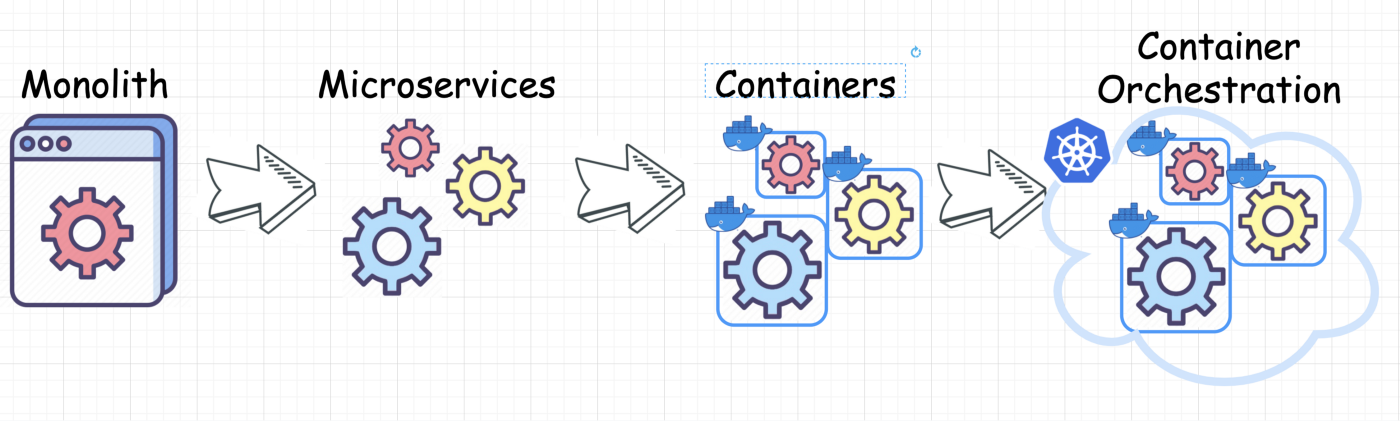
\includegraphics[width=0.8\textwidth]{resources/containerization.png}
      \caption{Από μονολιθικές εφαρμογές, στις μικροϋπηρεσίες, στα containers τα οποία διαχειρίζεται ένας Container Orchestrator}
\end{figure}

\section{Kubernetes: Βασικές αρχές}
Ο Kubernetes είναι ένας ενορχηστρωτής container ανοιχτού κώδικα. Αναπτύχθηκε
αρχικά εσωτερικά από την Google. Από το 2014, οπότε και έγινε λογισμικό ανοιχτού
κώδικα, ο Kubernetes έχει εξελιχθεί σε ένα από τα μεγαλύτερα και πιο δημοφιλή
έργα ανοιχτού κώδικα στον κόσμο. Έχει γίνει το πρότυπο API για τη διαχείριση
cloud-native εφαρμογών, με παρουσία σχεδόν σε κάθε υπολογιστικό νέφος.  Παρέχει
το λογισμικό που είναι απαραίτητο για την επιτυχή ανάπτυξη και διαχείριση
αξιόπιστων, κλιμακούμενων, κατανεμημένων συστημάτων.

\begin{figure}
      \centering
      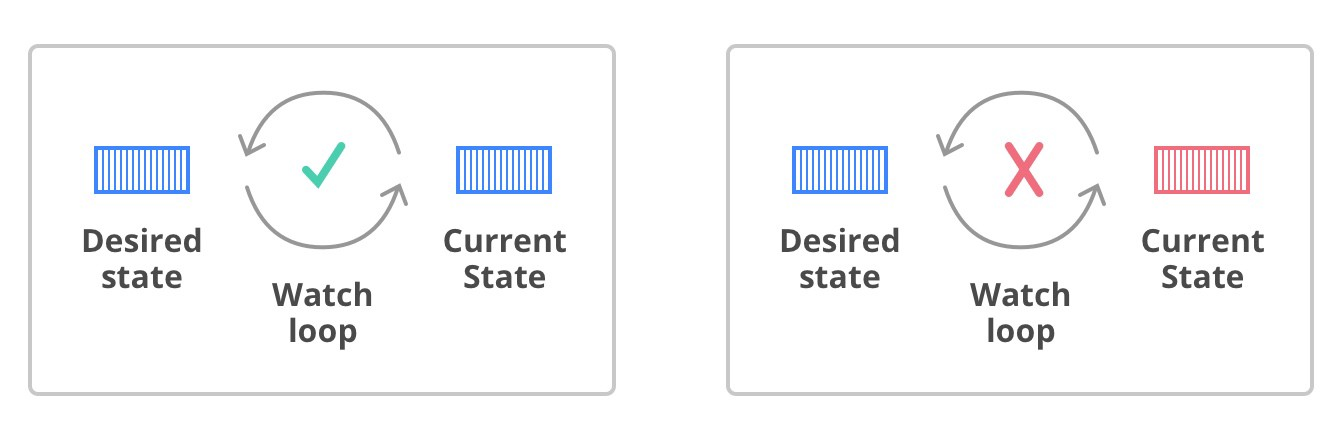
\includegraphics[width=0.8\textwidth]{resources/declarative.jpg}
      \caption{Ο βρόχος reconciliation του Kubernetes}
\end{figure}


Ο Kubernetes καθιστά τη διαχείριση του κύκλου ζωής των εφαρμογών που βασίζονται
σε containers πολύ πιο εύκολη, μέσω της δηλωτικής διαχείρισης της επιθυμητής
κατάστασης της συστοιχίας. Εκθέτει ένα ισχυρό δηλωτικό API, το οποίο οι
προγραμματιστές μπορούν να χρησιμοποιήσουν για να περιγράψουν την επιθυμητή
κατάσταση μιας εφαρμογής σε όρους Pods, Services, κ.λπ. και οι ελεγκτές του
Kubernetes θα εκτελέσουν άμεσα ενέργειες για να φέρουν την παρατηρούμενη
κατάσταση του συστήματος στην επιθυμητή κατάσταση.

\subsection{Η Αρχιτεκτονική του Kubernetes}

Μια συστοιχία Kubernetes αποτελείται από ένα σύνολο μηχανών εργασίας, που
ονομάζονται κόμβοι, οι οποίοι εκτελούν containerized εφαρμογές. Κάθε συστοιχία
διαθέτει τουλάχιστον έναν κόμβο εργασίας. Οι κόμβοι εργασίας φιλοξενούν τα Pods,
τα οποία είναι η μικρότερη μονάδα φορτίου εργασίας. Το επίπεδο ελέγχου
διαχειρίζεται τους κόμβους εργασίας και τα Pods στη συστοιχία. Σε περιβάλλοντα
παραγωγής, το επίπεδο ελέγχου εκτελείται συνήθως σε πολλούς υπολογιστές και μια
συστοιχία συνήθως λειτουργεί με πολλούς κόμβους, παρέχοντας ανοχή σε σφάλματα
και υψηλή διαθεσιμότητα.

\begin{figure}
      \centering
      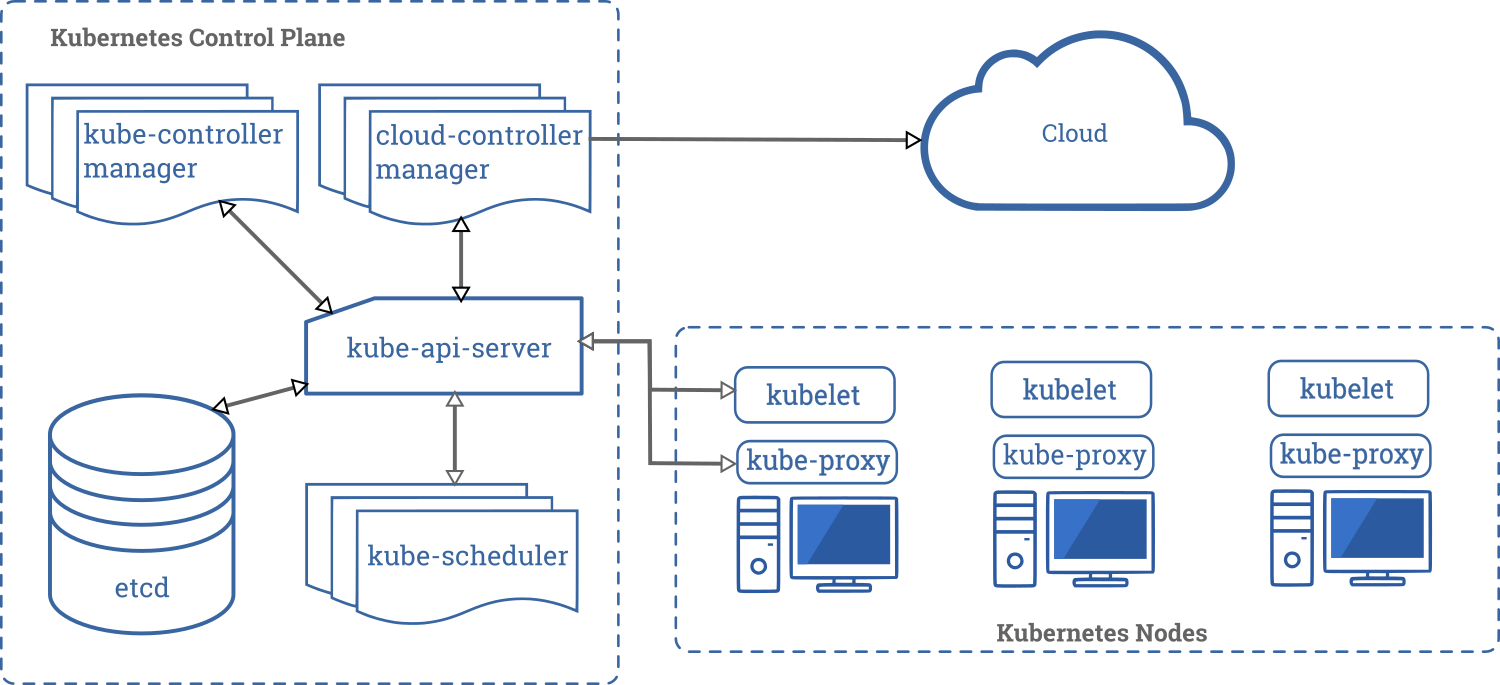
\includegraphics[width=\textwidth]{resources/components-of-kubernetes.png}
      \caption{H αρχιτεκτονική του Kubernetes}
\end{figure}

\subsection{Το API του Kubernetes}

Ο πυρήνας του επιπέδου ελέγχου του Kubernetes είναι ο  API Server. Ο  API Server
εκθέτει ένα HTTP API που επιτρέπει στους τελικούς χρήστες, σε διάφορα τμήματα
της συστοιχίας και σε εξωτερικούς στοιχεία να επικοινωνούν μεταξύ τους. Το API
του Kubernetes επιτρέπει στον χρήστη να υποβάλει ερωτήματα και να χειρίζεται
την κατάσταση των αντικειμένων API στον Kubernetes (για παράδειγμα: Pods,
Namespaces, ConfigMaps και Events).

Ο Kubernetes χρησιμοποιεί γενικά την κοινή ορολογία RESTful για να περιγράψει
τις έννοιες του API:
\begin{itemize}
      \tightlist
      \item Ένας \textit{τύπος πόρου} είναι το όνομα που χρησιμοποιείται στη
            διεύθυνση URL (Pods, Namespaces, Services).
      \item Όλοι οι τύποι πόρων έχουν μια συγκεκριμένη αναπαράσταση (το σχήμα
            του αντικείμενό τους) η οποία ονομάζεται \textit{είδος}.
      \item Μια λίστα από instances ενός πόρου είναι γνωστή ως \textit{συλλογή}.
      \item Ένα μεμονωμένο instance ενός τύπου πόρου ονομάζεται πόρος, και
            επίσης συνήθως αντιπροσωπεύει ένα αντικείμενο.
\end{itemize}

Σχεδόν όλοι οι τύποι πόρων αντικειμένων υποστηρίζουν τα τυπικά ρήματα HTTP -
\texttt{GET}, \texttt{POST}, \texttt{PUT}, \texttt{PATCH} και \texttt{DELETE}. Ο
Kubernetes χρησιμοποιεί επίσης τα δικά του ρήματα, τα οποία συχνά γράφονται με
μικρά γράμματα για να τα διακρίνει από τα ρήματα HTTP. Το Kubernetes
χρησιμοποιεί τον όρο ``\textit{list}'' για να περιγράψει την επιστροφή μίας
συλλογής πόρων και να τη διακρίνει από την ανάκτηση ενός μεμονωμένου πόρου που
ονομάζεται συνήθως ``\textit{get}''.

Όλοι οι τύποι πόρων είναι είτε \textit{cluster-scoped} από είτε σε ένα
\textit{namespace}.


\subsection{Τα Αντικείμενα του Kubernetes}

Τα \textit{αντικείμενα} του Kubernetes είναι μόνιμες οντότητες στο σύστημα. Ο
Kubernetes χρησιμοποιεί αυτές τις οντότητες για να αναπαριστά την κατάσταση της
συστοιχίας σας. Συγκεκριμένα, αυτά μπορούν να περιγράψουν:
\begin{itemize}
      \tightlist
      \item Ποιες containerized εφαρμογές εκτελούνται και σε ποιους κόμβους.
      \item Τους πόρους που είναι διαθέσιμοι σε αυτές τις εφαρμογές.
      \item Τις πολιτικές γύρω από τον τρόπο συμπεριφοράς αυτών των εφαρμογών,
            όπως οι πολιτικές επανεκκίνησης, αναβαθμίσεις και ανοχή σε σφάλματα.
\end{itemize}

Ένα αντικείμενο Kubernetes είναι μια ``\textit{καταγραφή της πρόθεσης}''. Μόλις
ένας χρήστης δημιουργήσει το αντικείμενο, το σύστημα του Kubernetes εργάζεται
διαρκώς για να διασφαλίζει την ύπαρξή του και να φέρει το σύστημα στην
επιθυμητή κατάσταση που έχει δηλώσει ο χρήστης.

\subsubsection{Το Αντικείμενο \co{Pod}}

Ένα \textit{Pod} αντιπροσωπεύει μια συλλογή από containers εφαρμογών και τους
τόμους τους, που τρέχουν στο ίδιο περιβάλλον εκτέλεσης. Τα Pods, και όχι τα
containers, είναι η μικρότερη μονάδα φορτίου εργασίας που μπορεί να εφαρμόσει ο
χρήστης σε μια συστοιχία του Kubernetes. Αυτό σημαίνει ότι όλα τα containers σε
ένα Pod καταλήγουν πάντα στο ίδιο μηχάνημα. Κάθε container μέσα σε ένα Pod
τρέχει στο δικό του cgroup, αλλά μοιράζονται έναν αριθμό namespaces του Linux.
Οι εφαρμογές που εκτελούνται στο ίδιο Pod μοιράζονται την ίδια διεύθυνση IP και
τον ίδιο χώρο θυρών (χώρος ονομάτων δικτύου), έχουν το ίδιο hostname (UTS
namespace) και μπορούν να επικοινωνούν χρησιμοποιώντας εγγενή κανάλια
επικοινωνίας μεταξύ διεργασιών μέσω System V IPC ή POSIX ουρές μηνυμάτων (IPC
namespace). Ωστόσο, οι εφαρμογές σε διαφορετικά Pods είναι απομονωμένες μεταξύ
τους - έχουν διαφορετικές διευθύνσεις IP, διαφορετικά hostnames, κ.λπ.

\paragraph*{Μη χρονοδρομολογήσιμα Pods}
Ο χρονοδρομολογητής της συστοιχίας είναι υπεύθυνος για την ανάθεση ενός κόμβου
για το Pod, ώστε να τρέξει σε αυτόν. Αυτό γίνεται με τον καθορισμό του πεδίου
\co{spec.nodeName} του Pod. Εάν ο χρονοδρομολογητής αποτυγχάνει να βρει ένα
μέρος για να τρέξει το Pod, θέτει το \co{PodScheduled} \co{PodCondition} σε
\co{False} και το reason σε \co{Unschedulable}. Ένα μη χρονοδρομολογήσιμος Pod
παραμένει στη φάση \co{Pending}.

Στο πλαίσιο της διπλωματικής εργασίας, θα αναφερόμαστε σε ένα Pod που δεν
μπόρεσε να χρονοδρομολογηθεί ως ``\textit{μη χρονοδρομολογήσιμο} Pod''.

\paragraph*{Αιτήματα πόρων και όρια}
\label{section:gr-pod-requests}

Οι υπολογιστικοί πόροι είναι μετρήσιμες ποσότητες που μπορούν να ζητηθούν, να
κατανεμηθούν, και να καταναλωθούν.

Ο χρήστης μπορεί να καθορίσει τα αιτήματα (requests) και τα όρια (limits) πόρων
για κάθε container του Pod. Ο χρονοδρομολογητής χρησιμοποιεί τα αιτήματα για να
αποφασίσει σε ποιον κόμβο θα τοποθετήσει το Pod. Το όρια ενός container,
χρησιμοποιούνται από το kubelet, το οποίο τα επιβάλλει, έτσι ώστε το τρέχον
container να μη χρησιμοποιήσει μεγαλύτερη ποσότητα του πόρου  από το όριο που
έχει ορίσει ο χρήστης στις προδιαγραφές του Pod. Το kubelet εξασφαλίζει επίσης
ότι για το κάθε container θα διαθέτει την ποσότητα των πόρων που αιτήθηκε. Εάν
ο κόμβος στον οποίο εκτελείται ένα Pod έχει αρκετή ποσότητα ενός πόρου
διαθέσιμη, είναι δυνατό (και επιτρέπεται) ένα container να χρησιμοποιήσει
περισσότερο πόρο από ό,τι ορίζει το αίτημά του για τον εν λόγω πόρο. Ωστόσο, ένα
container δεν επιτρέπεται να χρησιμοποιήσει περισσότερη ποσότητα από το όριο των
πόρων του.

\lstinputlisting[label={listing:gr-pod-requests},language=yaml,caption={Αιτήματα και όρια του container ενός Pod}]{code/pod-requests.yaml}

\subsubsection{Το Αντικείμενο \co{Node}} Ο Kubernetes εκτελεί το φορτίο εργασίας
τοποθετώντας Pods για να τρέξουν σε κόμβους. Ένας κόμβος μπορεί να είναι μία
εικονική ή φυσική μηχανή, ανάλογα με τη συστοιχία. Κάθε κόμβος διαχειρίζεται από
το επίπεδο ελέγχου, που περιέχει τις υπηρεσίες που είναι απαραίτητες για την
εκτέλεση των Pods. Ένας κόμβος που έχει εγγραφεί στη συστοιχία του Kubernetes
αναπαρίσταται με ένα Node αντικείμενο.

\paragraph*{Node taints}
Τα taints και τα tolerations είναι ένας μηχανισμός που μπορεί να χρησιμοποιηθεί
για να διασφαλιστεί ότι τα Pods δεν τοποθετούνται σε ακατάλληλους κόμβους.
Τα taints προστίθενται στους κόμβους, ενώ τα tolerations ορίζονται στις
προδιαγραφές του Pod. Όταν ένας χρήστης βάζει taint σε έναν κόμβο, αυτό θα
απωθεί όλα τα Pods εκτός από εκείνα που έχουν tolerations για το συγκεκριμένο
taint. Ένας κόμβος μπορεί να έχει ένα ή πολλά taints που σχετίζονται με αυτόν.

\paragraph*{Node allocatable}

Ως \textit{allocatable} ενός κόμβου ορίζεται η ποσότητα των υπολογιστικών
πόρων που είναι διαθέσιμοι για τα Pods.  Οι συνολικοί πόροι (χωρητικότητα) ενός
κόμβου μπορούν να κατηγοριοποιηθούν σε:

\begin{itemize}
      \tightlist
      \item \co{kube-reserved}: δεσμευμένοι πόροι για τους δαίμονες του
            συστήματος kubernetes όπως το kubelet, το container runtime, κ.λπ.
      \item \co{system-reserved}: δεσμευμένοι πόροι για δαίμονες του
            λειτουργικού συστήματος, όπως το ssh, το udevd, κλπ.
      \item \co{eviction-threshold}: καθορίζει τα όρια που ενεργοποιούν τις
            εξώσεις Pods όταν οι πόροι των κόμβων πέσουν κάτω από τη δεσμευμένη
            τιμή.
      \item \co{allocatable}: οι εναπομείναντες πόροι κόμβων που είναι
            διαθέσιμοι για τη χρονοδρομολόγηση των Pods.
\end{itemize}

\paragraph*{Node status}

Κάθε αντικείμενο Node έχει έναν subresource \texttt{/status} που υποδεικνύει την
κατάσταση του κόμβου. Η κατάσταση περιέχει πολλαπλές συνθήκες για τον κόμβο
και διαχειρίζεται από τον Node controller.

Στο πλαίσιο του Cluster Autoscaler και του Scheduler, ένας κόμβος
θεωρείται ``\textit{Unready}'' αν:
\begin{itemize}
      \tightlist
      \item Έχει το πεδίο \co{Pod.spec.unschedulable}. Αυτό το πεδίο υποδεικνύει
            ότι ο κόμβος δεν δέχεται νέα Pods.
      \item Το αντικείμενο του κόμβου δεν έχει καμία συνθήκη τύπου \co{Ready}.
      \item Υπάρχει μια συνθήκη τύπου \co{Ready} και η κατάστασή της είναι
            \co{False}.
      \item Μια συνθήκη τύπου \co{DiskPressure} ή \co{PIDPressure} ή
            \co{NetworkUnavailable} με την αντίστοιχη κατάστασή του να έχει
            οριστεί σε \co{True}. exists.
\end{itemize}
Οι υπόλοιποι κόμβοι θεωρούνται ``\textit{Ready}''.

Ένας κόμβος που δεν μπορεί να δεχτεί pods, θα αναφέρεται ως ``\textit{μη
      χρονοδρομολογήσιμος}'' κόμβος.


\subsubsection{Το Αντικείμενο \co{PodDisruptionBudget}}

Ένα \texttt{PodDisruptionBudget} (PDB) περιορίζει τον αριθμό των Pods μιας
replicated εφαρμογής που μπορούν να τεθούν εκτός λειτουργίας ταυτόχρονα από
εκούσιες διακοπές. Για το παράδειγμα, ένα web front end μπορεί να θέλει να
διασφαλίσει ότι ο αριθμός των αντιγράφων που εξυπηρετούν το φορτίο δεν πέφτει
ποτέ κάτω από ένα συγκεκριμένο ποσοστό του συνόλου.

Ένα PDB καθορίζει τον αριθμό των αντιγράφων που μπορεί να ανεχθεί να έχει μια
εφαρμογή, σε σχέση με τον αριθμό που προορίζεται να έχει. Για παράδειγμα, ένα
\co{Deployment} που έχει θέσει \texttt{.spec.replicas:\ 5} υποτίθεται ότι πρέπει
να έχει 5 Pods ανά πάσα στιγμή. Εάν το PDB του επιτρέπει να υπάρχουν 4 κάθε
φορά, τότε το Eviction API θα επιτρέψει εθελοντική διακοπή ενός (αλλά όχι δύο)
Pod κάθε φορά.

\subsubsection{Το Αντικείμενο \co{Deployment}}

Ένας αντικείμενο \co{Deployment} εξασφαλίζει ότι ένας συγκεκριμένος αριθμός Pod
\textit{replicas} εκτελείται ανά πάσα στιγμή. Με άλλα λόγια, ένα Deployment
διασφαλίζει ότι ένα Pod ή ένα ομοιογενές σύνολο Pods είναι πάντα σε λειτουργία
και διαθέσιμο. Εάν υπάρχουν περισσότερα Pods από όσα ζητούνται, θα σκοτώσει
μερικά. Αν υπάρχουν λιγότερα, ο Kubernetes θα δημιουργήσει πρόσθετα Pods.

\subsubsection{Το Αντικείμενο \co{DaemonSet}}

Ένας αντικείμενο \co{DaemonSet} (DS) διασφαλίζει ότι όλοι οι κόμβοι εκτελούν ένα
αντίγραφο ενός Pod. Καθώς οι κόμβοι προστίθενται στη συστοιχία, προστίθενται
Pods σε αυτούς. Καθώς οι κόμβοι αφαιρούνται από τη συστοιχία, αυτά τα Pods
γίνονται garbage collect. Η διαγραφή ενός DaemonSet θα αφαιρέσει τα Pods που
δημιούργησε.

\subsubsection{Το Αντικείμενο \co{PersistentVolumeClaim}}

Ένα αντικείμενο \co{PersistentVolumeClaim} (PVC, ή ισοδύναμα αναφέρεται ως
\textit{claim}) αναπαριστά ένα αίτημα ενός χρήστη για αποθηκευτικό χώρο.  Τα
PVCs μπορούν να ζητήσουν συγκεκριμένο μέγεθος χώρου αλλά και τρόπους πρόσβασης,
π.χ., \en{\co{ReadWriteOnce}}, \co{ReadOnlyMany} ή \co{ReadWriteMany}, κ.λπ.

\subsubsection{Το Αντικείμενο \co{PersistentVolume}}

Ένα \co{PersistentVolume} (PV, ή ισοδύναμα αναφέρεται ως \textit{τόμος})
αναπαριστά τόμο του αποθηκευτικού χώρου στη συστοιχία που έχει διατεθεί στατικά
από έναν διαχειριστή ή δυναμικά με τη χρήση κλάσεων αποθήκευσης. Τα PVs έχουν
έναν κύκλο ζωής ανεξάρτητο από κάθε μεμονωμένο Pod που χρησιμοποιεί το PV. Αυτό
το αντικείμενο API αποτυπώνει τις λεπτομέρειες του υλοποίησης του αποθηκευτικού
χώρου, είτε πρόκειται για NFS, iSCSI, είτε για ένα συγκεκριμένο σύστημα
αποθήκευσης.

\paragraph*{Δέσμευση}

Τα PVCs είναι αιτήσεις για πόρους αποθήκευσης - κάθε PVC δεσμεύεται σε ένα PV που
ταιριάζει με το ζητούμενο ποσό αποθήκευσης και τους τρόπους πρόσβασης του PVC.
Κάθε PV δεσμεύεται σε ένα μόνο PVC και αντίστροφα. Η δέσμευση μεταξύ τους είναι
αμφίδρομη.  Ένα PV θα παραμείνει αδέσμευτο έως ότου αντιστοιχιστεί σε ένα PVC.

\begin{figure}[ht]
      \centering
      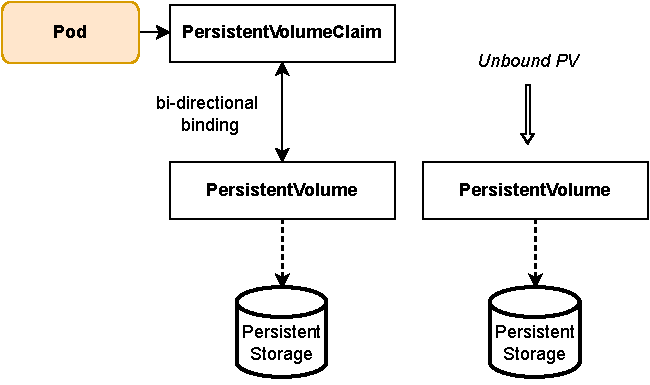
\includegraphics[width=0.8\textwidth]{resources/pvc-pv-binding.pdf}
      \caption{Ένα Pod ζητά έναν τόμο χρησιμοποιώντας ένα PVC και το PVC δεσμεύεται σε ένα PV. Το αντικείμενο PV αποθηκεύει τις λεπτομέρειες για το υποκείμενο κομμάτι μόνιμης αποθήκευσης.}
      \label{figure:gr-pvc-pv}
\end{figure}

\paragraph*{Node Affinity}

Κάθε αντικείμενο PersistentVolume έχα ένα node affinity, που υποδεικνύει του
κόμβους από τους οποίους είναι προσβάσιμος ο αντίστοιχος τόμος. Το
\co{nodeAffinity} πεδίο, είναι έναν επιλογέας ετικετών, ο οποίος επιλέγει
κόμβους με βάση τις ετικέτες τους.

Το node affinity ενός PV χρησιμοποιείται με τον ακόλουθο τρόπο για να υποδείξει
ότι ένας τόμος είναι τοπικός σε έναν κόμβο:
\begin{enumerate}
      \tightlist
      \item Ο οδηγός αποθήκευσης ορίζει σε κάθε αντικείμενο \texttt{Node} μια μοναδική
            ετικέτα.
      \item Ο οδηγός αποθήκευσης θέτει το αντίστοιχο node affinity του PV να
            ταιριάζει μόνο με τη μοναδική ετικέτα του κόμβου.
\end{enumerate}

\subsubsection{Το Αντικείμενο \co{StorageClass}}

Ένα \co{StorageClass} είναι ένας πόρος του Kubernetes που επιτρέπει τη δυναμική
παροχή τόμων. Ο διαχειριστής ρυθμίζει τις παραμέτρους του StorageClass. Ένα
StorageClass παρέχει έναν τρόπο στους διαχειριστές να περιγράψουν τις
``κλάσεις αποθήκευσης'' που προσφέρουν.

\subsection{Το Eviction API}


Κατά τη διαγραφή ενός πόρου στον Kubernetes, ο API Server θα βάλει ένα
\en{\co{deletionTimestamp}} στο αντικείμενο του πόρου, και αν δεν υπάρχουν
finalizers στο αντικείμενο, το αντικείμενο θα αφαιρεθεί από τον API Server.

Στην περίπτωση των Pods, εκτός από την κλασική λειτουργία \co{DELETE}, ο
Kubernetes προσφέρει ένα επιπλέον API για την έναρξη της διαγραφής του Pod: το
\co{Eviction} API. Η κύρια διαφορά με τη λειτουργία delete, είναι ότι οι
εκδιώξεις με πρωτοβουλία του API σέβονται τα ρυθμισμένα PodDisruptionBudgets και
\co{terminationGracePeriodSeconds}.

Έτσι, εάν ένας χρήστης προσπαθήσει να \textit{εκδιώξει} \footnote{Αναφερόμαστε
      στην έννοια \textit{eviction} με τον ελληνικό όρο ``\textit{εκδίωξη}''.} ένα Pod και
      το αντίστοιχο \en{PodDisruptionBudget} δεν επιτρέπει τη διατάραξη του Pod,
      το Pod δεν θα διαγραφεί. Αντίθετα, η εκτέλεση μιας κλασικής
      ενέργειας \co{DELETE}, θα αφαιρέσει το το Pod, ανεξάρτητα από το τι ορίζει
      το PodDisruptionBudget.

\subsection{Οι Διαδικασίες Cordon \& Drain}

Το CLI εργαλείο  \co{kubectl} του Kubernetes, επιτρέπει στον χρήστη να εκτελεί
εντολές σε συστοιχίες Kubernetes. Το εργαλείο επιτρέπει την πλήρη διαχείριση των
συστοιχιών. Δύο από τις πιο σημαντικές διαδικασίες που χρησιμοποιούνται για τη
συντήρηση μίας συστοιχίας είναι οι λειτουργίες \textit{cordon} και
\textit{drain}.

\paragraph*{Διαδικασία cordon}

Η διαδικασία \textit{cordon}, η οποία προσφέρεται από το CLI εργαλείο \co{kubectl},
χαρακτηρίζει έναν κόμβο ως \textit{μη χρονοδρομολογήσιμο}. Η επισήμανση ενός
κόμβου ως μη χρονοδρομολογήσιμου εμποδίζει τον χρονοδρομολογητή να τοποθετήσει
νέα Pods σε αυτόν τον κόμβο, αλλά δεν επηρεάζει τα υπάρχοντα Pods σε αυτόν. Αυτό
είναι χρήσιμο ως προπαρασκευαστικό βήμα πριν από την επανεκκίνηση του κόμβου ή
άλλη εργασία συντήρησης.

Ο διαχειριστής της συστοιχίας μπορεί να εκτελέσει τη διαδικασία cordon
εκτελώντας την εντολή \co{kubectl cordon}. Το εργαλείο προσθέτει το
\textit{unschedulable taint} \footnote{Unschedulable taint:
\co{node.kubernetes.io/unschedulable:NoSchedule}} στον κόμβο και θέτει επίσης το
πεδίο \co{nodes.spec.unschedulable} σε \co{True}.

\paragraph*{Διαδικασία drain}

Η διαδικασία \textit{drain} χρησιμοποιείται για την απομάκρυνση του φορτίου
εργασίας από έναν κόμβο, σε περίπτωση συντήρησης του κόμβου ή σε περίπτωση που
ένας κόμβος πρέπει να αφαιρεθεί εντελώς από ένα cluster. Η λειτουργία
αποστράγγισης θα κάνει cordon τον κόμβο για να τον χαρακτηρίσει ως μη
χρονοδρομολογήσιμο και θα εκδιώξει με ασφάλεια όλα τα Pods από τον κόμβο.  Οι
ασφαλείς εκδιώξεις επιτρέπουν στα containers του Pod να τερματίσουν
gracefully και σέβονται τα PodDisruptionBudgets που έχει ορίσει ο χρήστης.

Ο διαχειριστής της συστοιχίας μπορεί να εκτελέσει τη λειτουργία drain εκτελώντας
την εντολή \co{kubectl drain}. Εάν η εντολή επιστρέψει επιτυχώς, σημαίνει ότι
όλα τα Pods έχουν εκδιωχθεί με ασφάλεια, τηρώντας το PodDisruptionBudget που
έχει οριστεί. Στη συνέχεια, είναι ασφαλές να τερματιστεί ο κόμβος με την
απενεργοποίηση της φυσικής του μηχανής ή, αν εκτελείται σε πλατφόρμα
υπολογιστικού νέφους, διαγράφοντας την εικονική του μηχανή.

\section{Kubernetes Admission Webhooks}

Τα admission webhooks είναι HTTP callbacks που λαμβάνουν αιτήματα εισδοχής και
κάνουν κάτι με αυτά. Μπορούν να οριστούν δύο τύποι admission webhooks:
\textit{validating admission} webhook και \textit{mutating admission} webhook.

Τα mutating webhooks καλούνται πρώτα και μπορούν να τροποποιήσουν
αντικείμενα που αποστέλλονται στον API Server για την επιβολή προσαρμοσμένων
προεπιλογών. Αφού ολοκληρωθούν όλες οι τροποποιήσεις αντικειμένων, και αφού το
εισερχόμενο αντικείμενο επικυρωθεί από τον  API Server, καλούνται τα validating
webhooks και μπορούν να απορρίψουν αιτήσεις για την επιβολή συγκεκριμένων
πολιτικών αναφορικά με τα αντικείμενα που δημιουργούνται στη συστοιχία.

Ο διαχειριστής της συστοιχίας μπορεί να ρυθμίσει δυναμικά τι πόροι υπόκεινται σε
ποια webhooks μέσω των αντικειμένων \en{\co{ValidatingWebhookConfiguration}} ή
\en{\co{MutatingWebhookConfiguration}}.

\paragraph*{\co{MutatingWebhookConfiguration} Object}

Κάθε \texttt{MutatingWebhookConfiguration} περιέχει μια λίστα με webhooks, που
καθορίζονται στο πεδίο \co{webhooks}. Καθένα από τα webhooks που ορίζονται,
περιλαμβάνει τα ακόλουθα πεδία:

\begin{itemize}
      \tightlist
      \item \texttt{rules}: Μία λίστα κανόνων που χρησιμοποιούνται για να
            καθοριστεί εάν ένα αίτημα προς στον API Server θα πρέπει να
            σταλεί στο webhook.
      \item \texttt{failurePolicy}: Καθορίζει τον τρόπο με τον οποίο θα
            χειριστεί ο API Server ένα timeout error ή οποιοδήποτε άλλο σφάλμα
            του webhook. Οι επιτρεπόμενες τιμές είναι \texttt{Ignore} ή
            \texttt{Fail}.
      \item \texttt{namespaceSelector}:  Καθορίζει εάν θα εκτελεστεί το webhook
            σε ένα αντικείμενο βάσει του namespace στο οποίο ανήκει.
\end{itemize}

\section{Kubernetes Scheduler} \label{section:gr-background_scheduler}

\subsection{Χρονοδρομολόγηση: Βασικές Αρχές}
\label{section:gr-scheduling-fundamentals}

\paragraph*{Πολλαπλοί χρονοδρομολογητές}
Ένας χρονοδρομολογητής σε μία συστοιχία \en{Kubernetes} είναι ένα στοιχείο που
παρακολουθεί για πρόσφατα δημιουργημένα Pods που δεν έχουν ανατεθεί σε κάποιον
κόμβο. Για κάθε Pod που ο scheduler ανακαλύπτει, γίνεται υπεύθυνος για την
εύρεση του καλύτερου κόμβου για το συγκεκριμένο Pod για να εκτελεστεί.

Ο \co{kube-scheduler} είναι ο προεπιλεγμένος χρονοδρομολογητής για τον
Kubernetes και εκτελείται ως μέρος του επιπέδου ελέγχου. Ωστόσο, είναι πιθανό να
εκτελούνται πολλαπλοί χρονοδρομολογητές σε μια συστοιχία. Σε αυτή την περίπτωση
κάθε Pod πρέπει να καθορίσει στο spec του το όνομα του χρονοδρομολογητή που θα
το χειριστεί, θέτοντας στο πεδίο \co{spec.schedulerName} το όνομα του
προτιμώμενου scheduler. Εάν το Pod δεν έχει ορίσει ρητά το όνομα του
χρονοδρομολογητή, το Pod θα χρονοδρομολογηθεί χρησιμοποιώντας τον προεπιλεγμένο
χρονοδρομολογητή.

\paragraph*{Εφικτοί κόμβοι} Κάθε Pod έχει διαφορετικές απαιτήσεις, π.χ. CPU,
μνήμη, που επηρεάζουν σε ποιους κόμβους μπορεί να εκτελεστεί το Pod. Οι
παράγοντες που πρέπει να ληφθούν υπόψη για τις αποφάσεις χρονοδρομολόγησης
περιλαμβάνουν ατομικούς και συλλογικούς πόρους, περιορισμοί
υλικού/λογισμικού/πολιτικής, προτιμήσεις και μη προτιμήσεις κόμβων, τοπικότητα
δεδομένων, παρεμβολές μεταξύ φορτίων εργασίας, κ.λπ. Οι κόμβοι που πληρούν τις
απαιτήσεις χρονοδρομολόγησης για ένα Pod ονομάζονται \textit{}{εφικτοί} κόμβοι.
Εάν κανένας από τους κόμβους στη συστοιχία δεν είναι εφικτός, το Pod θα
παραμείνει \textit{μη χρονοδρομολογήσιμο}, δηλαδή δεν θα του ανατεθεί κάποιος
κόμβος για να τρέξει.

Ο προεπιλεγμένος χρονοδρομολογητής του Kubernetes επιλέγει έναν κόμβο για το Pod
σε μια διαδικασία 3 βημάτων:
\begin{enumerate}
      \tightlist
      \item \textit{Filtering}: ο χρονοδρομολογητής βρίσκει το σύνολο των κόμβων
            όπου είναι εφικτό να χρονοδρομολογηθεί το Pod. Εκτελεί μια σειρά από
            πρόσθετα φιλτραρίσματος, που αξιολογούν αν το Pod μπορεί να
            τοποθετηθεί στον εξεταζόμενο κόμβο. Για το παράδειγμα, το φίλτρο
            ``PodFitsResources'' ελέγχει αν ένας υποψήφιος κόμβος έχει αρκετούς
            διαθέσιμους πόρους (CPU, μνήμη, GPU) για να καλύψει τις αιτήματα
            πόρων του Pod. Ένας κόμβος είναι εφικτός εάν όλα τα πρόσθετα φίλτρων
            θεωρούν τον κόμβο ως εφικτό για το Pod. Αυτό το βήμα υπολογίζει μια
            λίστα κόμβων με κατάλληλους (εφικτούς) κόμβους. Αν η λίστα αυτή
            είναι κενή, το Pod δεν μπορεί να χρονοδρομολογηθεί σε κάποιον κόμβο
            (μη χρονοδρομολογήσιμο).
      \item \textit{Scoring}: ο χρονοδρομολογητής αποδίδει μία βαθμολογία σε
            κάθε εφικτό κόμβο και τους κατατάσσει για να επιλέξει τον πιο
            κατάλληλη τοποθέτηση Pod.
      \item Στη συνέχεια, ο χρονοδρομολογητής αναθέτει το Pod στον κόμβο με την
            υψηλότερη βαθμολογία. Εάν υπάρχουν περισσότεροι από ένας κόμβοι με
            ίση βαθμολογία, επιλέγει έναν από αυτούς τυχαία. Η ανάθεση το Pod σε
            έναν κόμβο γίνεται θέτοντας στο πεδίο \co{spec.nodeName} του Pod το
            όνομα του επιλεγμένου κόμβου.
\end{enumerate}


\subsection{Το Πλαίσιο Χρονοδρομολόγησης}

Το πλαίσιο χρονοδρομολόγησης είναι μια pluggable αρχιτεκτονική για τον
Kubernetes Scheduler. Προσθέτει ένα σύνολο από ``πρόσθετα'' APIs στον υπάρχοντα
χρονοδρομολογητή. Τα πρόσθετα μεταγλωττίζονται και είναι ενσωματωμένα στον
χρονοδρομολογητή. Τα APIs επιτρέπουν τα περισσότερα χαρακτηριστικά της
χρονοδρομολόγησης να υλοποιούνται ως πρόσθετα, διατηρώντας παράλληλα τον πυρήνα
του χρονοδρομολογητή ελαφρύ και συντηρήσιμο.

\paragraph*{Κύκλος χρονοδρομολόγησης \& κύκλος δέσμευσης}

Ο χρονοδρομολογητής διατηρεί μια ουρά με Pods που περιμένουν να
χρονοδρομολογηθούν. Διαλέγει ένα Pod από την ουρά και επιχειρεί να το
χρονοδρομολογήσει. Κάθε προσπάθεια χρονοδρομολόγησης ενός Pod χωρίζεται σε δύο
φάσεις:

\begin{itemize}
      \tightlist
      \item \textit{Κύκλος χρονοδρομολόγησης}: αποφασίζει έναν κόμβο για το Pod.
            Οι κύκλοι χρονοδρομολόγησης διαφορετικών Pods εκτελούνται σειριακά.
      \item \textit{Κύκλος δέσμευσης}: εφαρμόζει αυτή την απόφαση για το Pod στη
            συστοιχία. Πολλαπλοί κύκλοι δέσμευσης για διαφορετικά Pods
            εκτελούνται παράλληλα.
\end{itemize}

Ο κύκλος χρονοδρομολόγησης και ο κύκλος δέσμευσης αναφέρονται συνολικά ως
``\textit{scheduling context}''. Ένας κύκλος χρονοδρομολόγησης ή ένας κύκλος
δέσμευσης
μπορεί να διακοπεί εάν το Pod διαπιστωθεί ότι δεν μπορεί να ανατεθεί σε κανέναν
κόμβο ή αν υπάρξει κάποιο εσωτερικό σφάλμα. Το Pod θα επιστρέψει στην ουρά
αναμονής και θα γίνει προσπάθεια εκ νέου κάποια επόμενη στιγμή. Εάν ένας κύκλος
δέσμευσης ματαιωθεί, θα ενεργοποιήσει τη μέθοδο \texttt{Unreserve} των πρόσθετων
ώστε να απελευθερωθούν τυχόν πόροι που έχουν δεσμευτεί για το Pod και να
αναστραφούν τυχόν αποφάσεις που έχουν αποτυπωθεί στη συστοιχία.

Το πλαίσιο χρονοδρομολόγησης εκθέτει ορισμένα σημεία επέκτασης.  Τα πρόσθετα
εγγράφονται για να κληθούν σε ένα ή περισσότερα από αυτά τα σημεία επέκτασης.
Ένα πρόσθετο μπορεί να εγγραφεί σε πολλαπλά σημεία επέκτασης. Τα σημεία
επέκτασης παρουσιάζονται στο Σχήμα ~\ref{fig:scheduling-plugins-gr}.

\begin{figure}[ht]
      \centering
      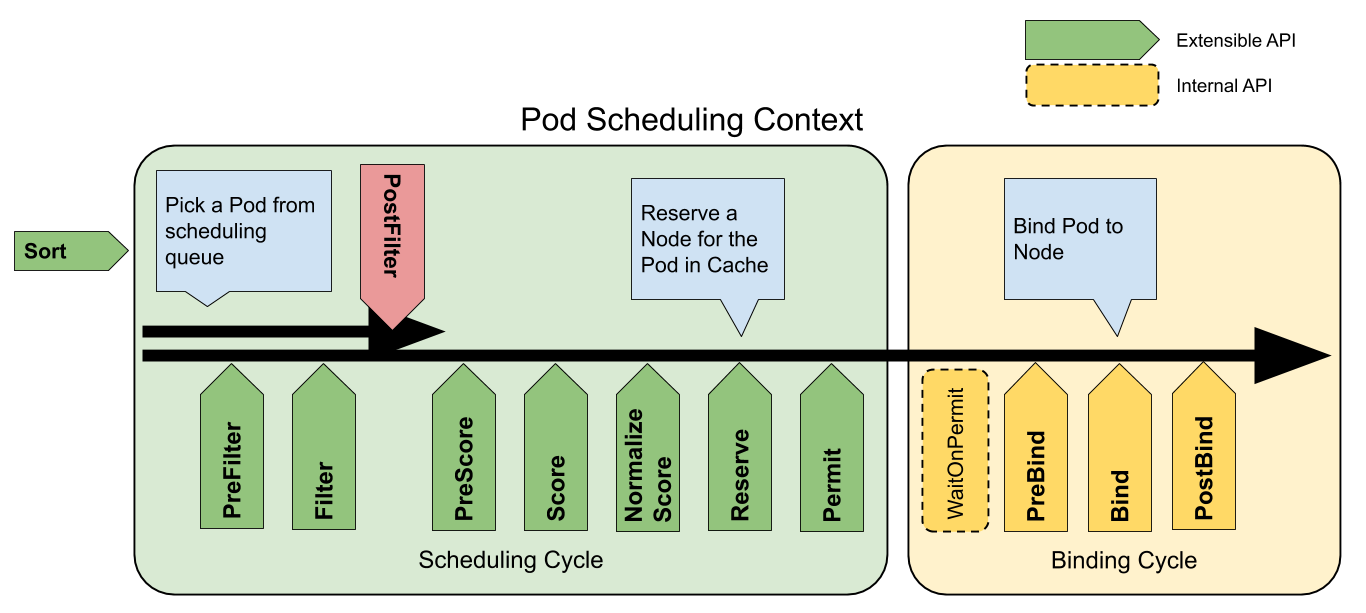
\includegraphics[width=\textwidth]{chapters/background/img/scheduler.png}
      \caption{Τα σημεία επέκτασης του πλαισίου χρονοδρομολόγησης}
      \label{fig:scheduling-plugins-gr}
\end{figure}


Το πλαίσιο του χρονοδρομολογητή προσφέρει τα ακόλουθα σημεία επέκτασης, όπου
κάθε πρόσθετο μπορεί να καταχωρηθεί:

\begin{itemize}
      \item
            \textbf{\co{Queue sort}}: Αυτά τα πρόσθετα χρησιμοποιούνται για την
            ταξινόμηση των Pods στην ουρά του scheduler. Ένα πρόσθετο
            ταξινόμησης ουράς ουσιαστικά θα παρέχει μια \texttt{less(pod1,
            Pod2)} συνάρτηση. Μόνο ένα πρόσθετο ταξινόμησης ουράς μπορεί να
            είναι ενεργοποιημένο.
      \item
            \textbf{\co{PreFilter}}: Αυτά τα πρόσθετα χρησιμοποιούνται για την
            προεπεξεργασία πληροφοριών σχετικά με το Pod, ή για να ελέγξουν
            ορισμένες συνθήκες που η συστοιχία ή το Pod πρέπει να πληρούν. Ένα
            πρόσθετο PreFilter θα πρέπει να υλοποιεί μια PreFilter μέθοδο. Εάν η
            PreFilter μέθοδος επιστρέψει σφάλμα, ο κύκλος χρονοδρομολόγησης
            ματαιώνεται.
      \item
            \textbf{\co{Filter}}: Αυτά τα πρόσθετα χρησιμοποιούνται για το
            φιλτράρισμα (αποκλεισμό) των κόμβων που δεν μπορούν να εκτελέσουν το
            Pod, και ισοδύναμα, για την εύρεση των κόμβων που μπορούν να
            φιλοξενήσουν ένα Pod (\textit{εφικτοί κόμβοι}). Για κάθε κόμβο, ο
            χρονοδρομολογητής θα καλέσει τα Filter πρόσθετα με τη σειρά που
            έχουν ρυθμιστεί. Εάν κάποιο πρόσθετο Filter χαρακτηρίσει τον κόμβο
            ως μη εφικτό, τα υπόλοιπα πρόσθετα δεν θα κληθούν για τον κόμβο
            αυτό. Οι κόμβοι μπορούν να αξιολογούνται ταυτόχρονα και, συνεπώς,
            ένα Filter πρόσθετο μπορεί να κληθεί περισσότερες από μία φορές στον
            ίδιο κύκλο χρονοδρομολόγησης.
      \item
            \textbf{\co{PostFilter}}: Αυτά τα πρόσθετα καλούνται μετά το Filter
            φάση, αλλά μόνο όταν δεν βρέθηκαν εφικτοί κόμβοι για το Pod. Τα
            πρόσθετα αυτά καλούνται με τη ρυθμισμένη σειρά τους. Εάν κάποιο από
            τα πρόσθετα PostFilter θεωρήσει τον κόμβο ως εφικτό για το Pod, τα
            υπόλοιπα πρόσθετα δεν θα κληθούν. Μια τυπική εφαρμογή του PostFilter
            είναι το preemption, που προσπαθεί να καταστήσει εφικτή τη
            χρονοδρομολόγηση ενός Pod  με το να εκδιώξει άλλα Pods από τον
            κόμβο.
      \item
            \textbf{\co{PreScore}}: Αυτό είναι ένα σημείο επέκτασης για το την
            εκτέλεση εργασιών προ-βαθμολόγησης. Τα πρόσθετα θα κληθούν με μια
            λίστα κόμβων που πέρασαν τη φάση Filter (εφικτοί κόμβοι). Ένα
            πρόσθετο μπορεί να χρησιμοποιήσει αυτά τα δεδομένα για να ενημερώσει
            την εσωτερική κατάσταση ή να δημιουργήσει αρχεία καταγραφής και να
            υπολογίσει διάφορες μετρικές.
      \item
            \textbf{\co{Scoring}}:
            \begin{itemize}
                  \item
                        Η πρώτη φάση ονομάζεται ``\textit{score}'' και
                        χρησιμοποιείται για την κατάταξη των κόμβων που έχουν
                        περάσει τη φάση φιλτραρίσματος. Ο χρονοδρομολογητής θα
                        καλέσει τη μέθοδο \texttt{Score} του κάθε προσθέτου
                        βαθμολόγησης για κάθε κόμβο.
                  \item
                        Η δεύτερη φάση ονομάζεται ``\textit{normalize scoring}''
                        και χρησιμοποιείται για την τροποποίηση των βαθμολογιών
                        πριν ο χρονοδρομολογητής υπολογίσει την τελική κατάταξη
                        των κόμβων.
            \end{itemize}

      \item
            \textbf{\co{Reserve}}: Ένα πρόσθετο που υλοποιεί την επέκταση
            Reserve έχει δύο μεθόδους, συγκεκριμένα τις \texttt{Reserve} και
            \texttt{Unreserve}. Τα πρόσθετα που διατηρούν την κατάσταση
            εκτέλεσης (\textit{stateful πρόσθετα}) θα πρέπει να χρησιμοποιούν
            αυτές τις φάσεις για να ειδοποιούνται από τον χρονοδρομολογητή όταν
            οι πόροι σε έναν κόμβο δεσμεύονται και αποδεσμεύονται για ένα
            συγκεκριμένο Pod. 
            
            Η φάση \emph{Reserve} υπάρχει για να αποτρέψει συνθήκες ανταγωνισμού
            ενώ ο χρονοδρομολογητής περιμένει να πετύχει η δέσμευση. Εκτελείται
            πριν ο χρονοδρομολογητής δεσμεύσει πραγματικά ένα Pod στον
            καθορισμένο κόμβο. Η μέθοδος Reserve μπορεί να επιτύχει ή να
            αποτύχει.
            
            Εάν η μέθοδος \texttt{Reserve} όλων των πρόσθετων στοιχείων πετύχει,
            η φάση Reserve θεωρείται επιτυχής και το υπόλοιπο του κύκλου
            χρονοδρομολόγησης και ο κύκλος δέσμευσης εκτελούνται.

            Αν μια κλήση της μεθόδου \texttt{Reserve} ενός προσθέτου αποτύχει,
            τα επόμενα πρόσθετα δεν εκτελούνται και η φάση Reserve θεωρείται
            αποτυχημένη. Τότε, ο χρονοδρομολογητής θα καλέσει τη φάση
            \co{Unreserve}. Η  \co{Unreserve}  φάση υπάρχει για να καθαρίσει την
            κατάσταση που σχετίζεται με τις δεσμεύσεις ενός Pod. Όταν συμβαίνει
            αυτό, οι μέθοδοι \texttt{Unreserve} όλων των \texttt{Reserve}
            προσθέτων θα εκτελεστούν με την αντίστροφη σειρά από αυτή των
            κλήσεων των μεθόδων \texttt{Reserve}.
            
      \item
            \textbf{\co{Permit}}: Αυτά τα πρόσθετα χρησιμοποιούνται για να
            αποτρέψουν ή να καθυστερήσουν τη δέσμευση ενός Pod. Τα πρόσθετα
            Permit εκτελούνται ως το τελευταίο βήμα ενός κύκλου
            χρονοδρομολόγησης, ωστόσο η αναμονή στη φάση της άδειας συμβαίνει
            κατά την αρχή ενός κύκλου δέσμευσης, πριν εκτελεστούν τα πρόσθετα
            PreBind.
\end{itemize}


\subsection{To Πρόσθετο VolumeBinding}


Το πρόσθετο \texttt{VolumeBinding} είναι ένα πρόσθετο του Kubernetes Scheduler
που δεσμεύει τους τόμους Pod κατά τη χρονοδρομολόγηση. Το πρόσθετο VolumeBinding
είναι εγγεγραμμένο στα PreFilter, Filter, PreBind, Reserve, Unreserve σημεία
επέκτασης του πλαισίου χρονοδρομολόγησης.

Ιδιαίτερο ενδιαφέρον στο πλαίσιο της παρούσας διπλωματικής εργασίας παρουσιάζουν
οι PreFilter, Filter, PreBind φάσεις του πρόσθετου, επομένως εξηγούμε εδώ εν
συντομία τις λειτουργίες που λαμβάνουν χώρα:

\begin{itemize}
      \tightlist
      \item \co{PreFilter}: ελέγχει αν από τα PVCs που αναφέρει το Pod, τα PVC
            με “immediate”  binding mode, είναι δεσμευμένα με κάποιο PV. Εάν δεν
            ικανοποιείται αυτή η συνθήκη, επιστρέφεται σφάλμα.
      \item \co{Filter}: αξιολογεί αν ένα Pod μπορεί να τοποθετηθεί σε έναν
            κόμβο, βάσει των τόμων που ζητά, τόσο για τα δεσμευμένα όσο και για
            τα μη δεσμευμένα PVC:
            \begin{itemize}
                  \tightlist
                  \item Για τα \textit{δεσμευμένα PVC}, ελέγχει ότι το PV του
                        κάθε PVC είναι προσβάσιμο (βάσει τoy node affinity που
                        φέρει) από τον εξεταζόμενο κόμβο.
                  \item Για τα \textit{μη δεσμευμένα PVC}, προσπαθεί να βρει
                        διαθέσιμα PVs που μπορούν να ικανοποιήσουν τις
                        απαιτήσεις του PVC και που είναι προσβάσιμα (βάσει του
                        node affinity τους) από τον εξεταζόμενο κόμβο. Εάν δεν
                        βρει κατάλληλα PVs, αναλαμβάνει να ενημερώσει με τα
                        κατάλληλα annotations τον οδηγό, ώστε να γίνει δυναμική
                        παροχή των τόμων.
                  \item Εάν είναι ενεργοποιημένη η παρακολούθηση της
                        χωρητικότητας αποθήκευσης, ελέγχει εάν υπάρχει αρκετός
                        χώρος διαθέσιμος από τον κόμβο για τους τόμους που
                        πρέπει να δημιουργηθούν στο σύστημα αποθήκευσης.
                  \item Το πρόσθετο επιστρέφει \texttt{true} αν όλα τα
                        δεσμευμένα PVC έχουν συμβατά PV με τον κόμβο και αν όλα
                        τα μη δεσμευμένα PVC μπορούν να αντιστοιχιστούν με ένα
                        διαθέσιμο και προσβάσιμο από τον κόμβο PV ή αν τα μη
                        δεσμευμένα μπορούν να δημιουργηθούν δυναμικά και να
                        αντιστοιχιστούν εν συνεχεία με το αντίστοιχο PV (dynamic
                        provision).
            \end{itemize}
      \item \co{PreBind}: Η PreBind μέθοδος θα ενημερώσει τον API Server με τις
            δεσμεύσεις (bindings) που υπολόγισε στα προηγούμενα βήματα και θα
            περιμένει έως ότου ο ελεγκτής PersistentVolume ολοκληρώσει πλήρως τη
            δέσμευση (bidirectional binding PV-PVC). Εάν η δέσμευση παρουσιάσει
            σφάλμα, λήξει ο χρόνος ή αναιρεθεί, τότε θα εμφανιστεί ένα σφάλμα
            και το Pod θα επιστραφεί στην ουρά για να επαναληφθεί η
            χρονοδρομολόγηση.
\end{itemize}


\section{Kubernetes Cluster Autoscaler}

Υπάρχουν 3 διαφορετικοί τύποι αυτόματης κλιμάκωσης στον Kubernetes:
\begin{itemize}
      \tightlist
      \item \textbf{Cluster Autoscaler (Autoscaler)}: ρυθμίζει τον αριθμό των
            κόμβων στη συστοιχία όταν τα Pods αποτυγχάνουν να χρονοδρομολογηθούν
            ή όταν οι κόμβοι υποχρησιμοποιούνται.
      \item \textbf{Horizontal Pod Autoscaler (HPA)}: ρυθμίζει τον αριθμό
            (replicas) των αντιγράφων μιας εφαρμογής που τρέχουν στη συστοιχία.
      \item \textbf{Vertical Pod Autoscaler (VPA)}: προσαρμόζει τους αιτούμενους
            πόρους και τα όρια των πόρων των container ενός Pod.
\end{itemize}

Στο πλαίσιο αυτής της διπλωματικής εργασίας συζητάμε μόνο για τον Cluster
Autoscaler. Ο Cluster Autoscaler προσαρμόζει το μέγεθος της συστοιχίας του
Kubernetes με βάση τους πόρους που αιτούνται από τα Pods και το ποσοστό
αξιοποίησης των πόρων του κάθε κόμβου στη συστοιχία. Ο Cluster Autoscaler
προσθέτει ή αφαιρεί αυτόματα κόμβους σε μια συστοιχία με βάση τα αιτήματα πόρων
από τα Pods. Σε καμία περίπτωση δεν μετράει ζωντανά τις τιμές χρήσης της CPU και
της μνήμης του Pod για να λάβει μια απόφαση κλιμάκωσης, αλλά, αντ' αυτού
βασίζεται αποκλειστικά στα αιτήματα του Pod για CPU και μνήμη.

\subsection{Αυτόματη Κλιμάκωση: Βασικές Αρχές}

Εάν υπάρχουν Pods στη συστοιχία που δεν μπόρεσαν να χρονοδρομολογηθούν από τον
Scheduler, (βρίσκονται σε κατάσταση \co{Pending}), o Autoscaler θα προσθέσει
έναν νέο κόμβο στη συστοιχία για να βοηθήσει το Pod να τρέξει. Αυτή η ενέργεια
ονομάζεται ``κλιμάκωση προς τα πάνω'' (scale-up) της συστοιχίας. Μόλις προστεθεί
ο κόμβος στη συστοιχία, ο Scheduler θα  αναθέσει το Pod στον κόμβο αυτό και θα
τρέξει.

Εάν υπάρχουν κόμβοι στη συστοιχία που δεν χρειάζονται, ο Autoscaler θα αφαιρέσει
αυτούς τους κόμβους. Αυτή η ενέργεια ονομάζεται ``κλιμάκωση προς τα κάτω''
(scale-down) της συστοιχίας.

Στις επόμενες παραγράφους θα εξηγήσουμε τις βασικές αρχές λειτουργίας του
Autoscaler.

\subsection{Διαδικασία Κλιμάκωσης Προς Τα Πάνω}
Ο Autoscaler ελέγχει περιοδικά για τυχόν Pods που δεν μπορούν να
χρονοδρομολογηθούν (κατάσταση Pending) και, εάν υπάρχουν, προσπαθεί να βρει έναν
νέο κόμβο με επαρκείς πόρους που θα μπορούσαν να τοποθετηθούν για να τρέξουν.

\begin{figure}[ht]
      \centering
      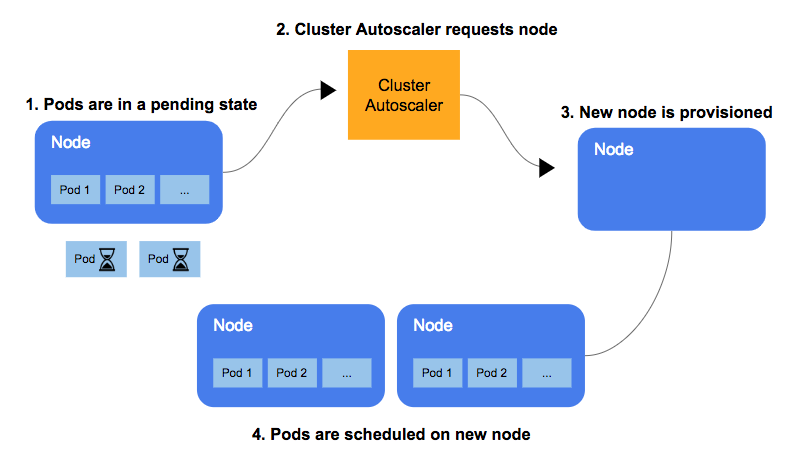
\includegraphics[width=\textwidth]{resources/autoscaler-scale-up.png}
      \caption{Διαδικασία κλιμάκωσης του Autoscaler}
\end{figure}

Ο Autoscaler υποθέτει ότι η υποκείμενη συστοιχία αποτελείται από κάποια είδη
ομάδων κόμβων. Μέσα σε μία ομάδα κόμβων, όλοι οι κόμβοι έχουν την ίδια ποσότητα
CPU και μνήμης και έχουν το ίδιο σύνολο εκχωρημένων ετικετών. Έτσι, αυξάνοντας
το μέγεθος μίας ομάδας κόμβων θα δημιουργήσει μια νέα μηχανή που θα είναι
παρόμοια με αυτές που βρίσκονται ήδη στη συστοιχία.

Με βάση την παραπάνω παραδοχή, ο Cluster Autoscaler δημιουργεί πρότυπα κόμβους
για κάθε ομάδα κόμβων και ελέγχει αν κάποιο από τα μη χρονοδρομολογήσιμα
Pods θα χωρούσε σε έναν νέο κόμβο της ομάδας. Εάν μετά από αυτή την αξιολόγηση
υπάρχουν πολλαπλές ομάδες κόμβων που, εάν αυξηθούν, θα βοηθούσαν στην εκτέλεση
των μη χρονοδρομολογήσιμων Pod, μπορούν να εφαρμοστούν διαφορετικές στρατηγικές
για την επιλογή της ομάδας κόμβων της οποίας το πλήθος κόμβων θα αυξηθεί.

\subsection{Διαδικασία Κλιμάκωσης Προς Τα Κάτω}

Ο Autoscaler ελέγχει περιοδικά, υπό την προϋπόθεση ότι δεν απαιτείται κλιμάκωση
προς τα πάνω, ποιοι κόμβοι δεν είναι απαραίτητοι. Ένας κόμβος θεωρείται μη
απαραίτητος προς αφαίρεση όταν ισχύουν όλες οι παρακάτω συνθήκες:

\begin{itemize}
      \tightlist
      \item Το άθροισμα των αιτήσεων CPU και μνήμης όλων των Pods που
            εκτελούνται σε αυτόν τον κόμβο είναι μικρότερο από το 50\% των
            διατιθέμενων πόρων του κόμβου (ο κόμβος υποχρησιμοποιείται). Το
            κατώφλι αυτό είναι προσαρμόσιμο.
      \item Όλα τα Pods που εκτελούνται στον κόμβο μπορούν να μετακινηθούν σε
            άλλους κόμβους. Κατά τον έλεγχο αυτής της συνθήκης, οι νέες θέσεις
            όλων των μετακινούμενων Pods απομνημονεύονται. Με αυτό τον τρόπο, ο
            Cluster Autoscaler γνωρίζει πού μπορεί να μετακινηθεί κάθε Pod και
            ποιοι κόμβοι εξαρτώνται από ποιους άλλους κόμβους όσον αφορά τη
            μετακίνηση Pod.

\end{itemize}

Εάν ένας κόμβος είναι μη απαραίτητος για περισσότερο από 10 λεπτά (προσαρμόσιμη
διάρκεια), θα τερματιστεί και θα αφαιρεθεί από τη συστοιχία. Ο Cluster
Autoscaler τερματίζει έναν \textit{μη κενό} κόμβο κάθε φορά για να μειώσει τον
κίνδυνο δημιουργίας μη χρονοδρομολογήσιμων Pods. Οι \textit{άδειοι} κόμβοι
(κόμβοι που τρέχουν μόνο DaemonSet Pods) μπορούν να τερματιστούν μαζικά.

Όταν τερματίζεται ένας μη κενός κόμβος, όπως αναφέρθηκε παραπάνω, όλα τα Pods θα
πρέπει να μεταφερθούν αλλού. Ο Autoscaler επιτυγχάνει να μετακινήσει τα Pods
αλλού ως εξής:
\begin{enumerate}
      \item Σημειώνει τον κόμβο στον API Server ως μη χρονοδρομολογήσιμο (δεν
            επιτρέπεται να χρονοδρομολογηθούν Pods σε αυτόν).
      \item Για κάθε Pod του κόμβου, στέλνει αίτημα εκδίωξης στον API Server.
\end{enumerate}



\section{Το Container Storage Interface}

Το Container Storage Interface  (CSI) είναι ένα πρότυπο για την έκθεση
συστημάτων block αποθήκευσης και συστημάτων αποθήκευσης αρχείων σε φορτία
εργασίας που τρέχουν σε containers, τα οποία διαχειρίζεται ένας ενορχηστρωτής
containers (Container Orchestrator - COs) όπως ο Kubernetes. Χρησιμοποιώντας το
CSI οι πάροχοι αποθήκευσης τρίτων μπορούν να γράψουν και να αναπτύσσουν plugins
που εκθέτουν νέα συστήματα αποθήκευσης στον Kubernetes χωρίς ποτέ να χρειαστεί
να αγγίξουν τον βασικό κώδικα του Kubernetes.

\subsection{Αρχιτεκτονική CSI Οδηγών}
Ένας CO αλληλεπιδρά με ένα CSI driver Plugin μέσω κλήσεων απομακρυσμένων
διαδικασιών (RPC). Κάθε CSI driver αποτελείται από τα ακόλουθα plugins:

\begin{itemize}
      \tightlist
      \item
            \textbf{Node Plugin}: Ένα gRPC endpoint που εξυπηρετεί CSI RPCs που
            χρειάζεται να εκτελεστούν στον κόμβο όπου θα δημοσιευτεί ο τόμος
            που ζητείται.
      \item
            \textbf{Controller Plugin}: Ένα  gRPC endpoint που εξυπηρετεί CSI
            RPCs που μπορούν να εκτελεστούν οπουδήποτε.
\end{itemize}

\begin{figure}[ht]
      \centering
      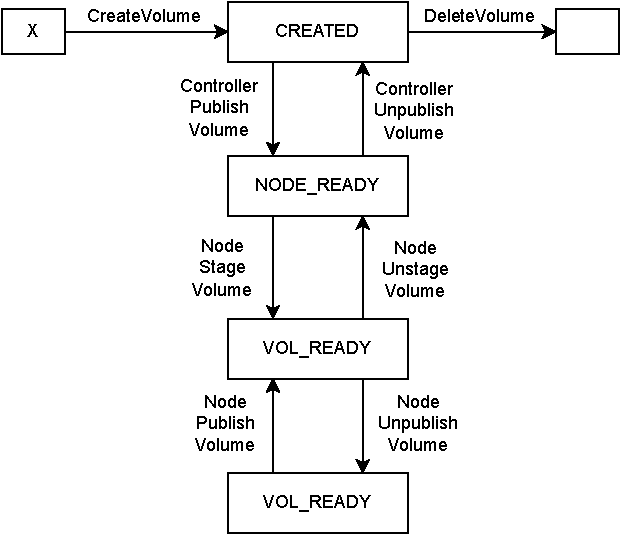
\includegraphics[width=0.7\textwidth]{resources/csi-states.pdf}
      \caption{Ο κύκλος ζωής ενός δυναμικά δημιουργούμενου τόμου, από τη δημιουργία μέχρι τη διαγραφή του}
      \label{figure:csi-lifecycle-gr}
\end{figure}

\subsection{CSI Remote Procedure Calls}

Το Container Storage Interface ορίζει τις RPCs που χρησιμοποιεί ένας
ενορχηστρωτής containers προκειμένου να αλληλεπιδράσει με τον οδηγό αποθήκευσης.
Κάθε μία από τις RPCs είναι μια idempotent λειτουργία. Η σειρά με την οποία
μπορούν να εκδοθούν οι κλήσεις παρουσιάζεται στο Σχήμα
\ref{figure:csi-lifecycle-gr}. Η λίστα των διαθέσιμων RPCs είναι η ακόλουθη:

\begin{itemize}

      \item{\co{CreateVolume}}: Ο external provisioner υποβάλλει αυτή την RPC
            στο CSI Controller service, ζητώντας του να παρέχει έναν νέο τόμο
            για έναν χρήστη. Εάν το πρόσθετο δεν είναι σε θέση να ολοκληρώσει
            την \co{CreateVolume} με επιτυχία, πρέπει να επιστρέψει ένα non-OK
            gRPC code.


            Ιδιαίτερο ενδιαφέρον στο πλαίσιο της παρούσας διπλωματικής εργασίας
            παρουσιάζει ο \co{RESOURCE\_EXHAUSTED} κωδικός. Με αυτόν τον κωδικό,
            υποδεικνύει ότι δεν μπορεί να παράσχει τον αιτούμενο τόμο με τους
            καθορισμένους περιορισμούς τοπολογίας, ενδεχομένως λόγω ανεπαρκούς
            χωρητικότητας αποθήκευσης.

      \item{\co{ControllerPublishVolume}}: Ο external attacher υποβάλλει αυτή
            την RPC στο CSI Controller service όταν ο Kubernetes θέλει να
            τοποθετήσει ένα φορτίο εργασίας που χρησιμοποιεί τον (ήδη
            provisioned) τόμο σε ένα κόμβο. To πρόσθετο θα πρέπει να εκτελέσει
            την απαραίτητη εργασία για να καταστήσει τον τόμο διαθέσιμο στο
            συγκεκριμένο κόμβο.

      \item{\co{NodeStageVolume}}:  Το kubelet υποβάλλει αυτή την RPC στο CSI
            Node service όταν ο τόμος πρόκειται να χρησιμοποιηθεί από το πρώτο
            Pod στον κόμβο. Πρέπει να εκτελείται μόνο μετά την επιτυχή εκτέλεση
            της \co{NodePublishVolume}. Ουσιαστικά χρησιμοποιείται για να
            μορφοποιηθεί ο τόμος και να προσαρτηθεί σε ένα staging directory του
            κόμβου.

      \item{\co{NodePublishVolume}}: Το kubelet υποβάλλει αυτή την RPC στο CSI
            Node service όταν ένα Pod ξεκινά να εκτελείται σε έναν κόμβο.
            Ουσιαστικά προσαρτά τον τόμο στον κατάλογο του Pod.

      \item{\co{NodeUnpublishVolume}}: Το kubelet υποβάλλει αυτή την RPC στο CSI
            Node service για να αναιρέσει την εργασία που έχει γίνει από την
            αντίστοιχη \co{NodePublishVolume}. Ουσιαστικά αποπροσαρτά τον τόμο
            από το κατάλογο του Pod.

      \item{\co{NodeUnstageVolume}}: Το kubelet υποβάλλει αυτή την RPC προς τον
            CSI Node service για να αναιρέσει την εργασία του αντίστοιχου
            \co{NodeStageVolume}. Ουσιαστικά, αποπροσαρτά τον τόμο από τον
            κατάλογο staging του κόμβου.

      \item{\co{ControllerUnpublishVolume}}: Ο external attacher υποβάλλει αυτή
            την RPC στο CSI Controller service για να εκτελέσει τις εργασίες που
            είναι απαραίτητες για να καταστήσει τον τόμο έτοιμο να
            καταναλωθεί από έναν διαφορετικό κόμβο. Αυτή η κλήση αναιρεί κάθε
            εργασία που έχει γίνει από την \\en{co{ControllerPublishVolume}}.

      \item{\co{DeleteVolume}}: Ο  external provisioner υποβάλλει αυτή την RPC στο
            CSI Controller service για να καταργήσει την παροχή ενός τόμου.
            Είναι η αντίστροφη λειτουργία της \co{CreateVolume}.

\end{itemize}

\section{Διαχείριση Λογικών Τόμων}

Η διαχείριση λογικών τόμων επιτρέπει το συνδυασμό πολλαπλών μεμονωμένων σκληρών
δίσκων ή/και κατατμήσεων δίσκου σε μια ενιαία ομάδα τόμων. Αυτή η ομάδα τόμων
μπορεί στη συνέχεια να υποδιαιρεθεί σε λογικούς τόμους (LV) ή να χρησιμοποιηθεί
ως ένας ενιαίος τόμος. Στη συνέχεια, μπορούν να δημιουργηθούν συστήματα αρχείων,
όπως EXT3 ή EXT4, σε κάθε λογικό τόμο.


Ο διαχειριστής λογικών τόμων (LVM) εισάγει ένα επιπλέον επίπεδο μεταξύ των
φυσικών δίσκων και του συστήματος αρχείων επιτρέποντας στα συστήματα αρχείων να:
\begin{itemize}
      \tightlist
      \item
            Αλλάζουν μέγεθος και να μετακινούνται εύκολα, χωρίς να απαιτείται
            διακοπή της λειτουργίας σε όλο το σύστημα.
      \item
            Χρησιμοποιούν ασυνεχή τμήματα χώρου στο δίσκο.
      \item
            Έχουν ουσιώδη ονόματα για τους τόμους, αντί για τα συνηθισμένα
            κρυπτογραφημένα ονόματα συσκευών.
      \item
            Επεκτείνονται σε πολλαπλούς φυσικούς δίσκους.
\end{itemize}


Το LVM αποτελείται από μερικά εννοιολογικά επίπεδα, όπως ο φυσικός τόμος, ο
λογικός τόμος και τα συστήματα αρχείων. Τα εννοιολογικά επίπεδα αποτελούνται με
τη σειρά τους από μικρότερες μονάδες όπως οι φυσικές εκτάσεις (στην περίπτωση
των φυσικών τόμων) και οι λογικές εκτάσεις (στην περίπτωση των λογικών τόμων).
\\
\begin{figure}[ht]
      \centering
      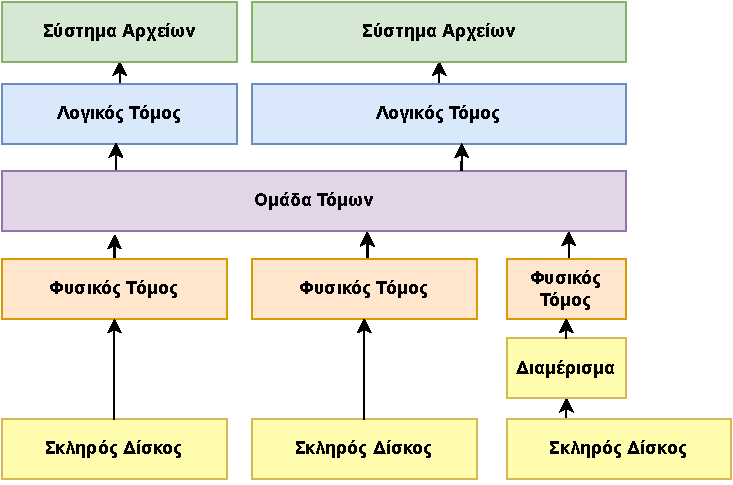
\includegraphics[width=0.8\textwidth]{resources/lvm-gr.pdf}
      \caption{Τα επίπεδα της διαχείρισης λογικών τόμων}
\end{figure}

\begin{itemize}
      \item \textbf{Φυσικός Τόμος}: Κάθε φυσικός τόμος μπορεί να είναι ένα
            διαμέρισμα δίσκου, ολόκληρος δίσκος, μία μετα-συσκευή ή ένα loopback
            αρχείο.
      \item \textbf{Ομάδα Τόμων}: Μια ομάδα τόμων συγκεντρώνει μια συλλογή από
            λογικούς τόμους και φυσικούς τόμους σε μια διοικητική μονάδα. Η
            ομάδα τόμων χωρίζεται σε ομάδες σταθερού μεγέθους που αποκαλούνται
            φυσικές εκτάσεις. Οι ομάδες τόμων αποτελούνται από φυσικούς τόμους,
            τα οποία με τη σειρά τους αποτελούνται από φυσικές εκτάσεις.
      \item \textbf{Λογικός Τόμος}: Ένας λογικός τόμος είναι το εννοιολογικό
            ισοδύναμο μιας κατάτμησης δίσκου σε ένα μη-LVM σύστημα. Οι λογικοί
            τόμοι είναι συσκευές μπλοκ οι οποίες δημιουργούνται από τις φυσικές
            εκτάσεις που υπάρχουν στην ίδια ομάδα τόμων.
\end{itemize}

\section{Το Λογισμικό Rok της Arrikto}

Το Rok παρέχει ένα επίπεδο διαχείρισης δεδομένων που καθιστά δυνατό για τους
χρήστες να δημιουργούν στιγμιότυπα των containers τους για τοπικά και εξωτερικά
αντίγραφα ασφαλείας, να λαμβάνουν αναλλοίωτα, ομαδικά συνεπή στιγμιότυπα των
εφαρμογών τους και να διατηρούν αυτά τα στιγμιότυπα σε ένα αποθετήριο αντιγράφων
ασφαλείας, π.χ. στο Amazon S3. Επιτρέπει στους χρήστες να δημιουργούν
στιγμιότυπα, εκδόσεις, πακέτα, να διανέμουν και να κλωνοποιούν το πλήρες
περιβάλλον τους μαζί με τα δεδομένα του. Είναι εγγενώς ενσωματωμένο με το
Kubernetes ως μία από τις υποστηριζόμενες πλατφόρμες του.

\subsection{Ο Rok Operator}

Οι συστοιχίες Rok συνοδεύονται από το \textit{Rok operator}, ένα στοιχείο που
 υλοποιεί τον Kubernetes \textit{operator pattern}  και διαχειρίζεται τη
 συστοιχία. Ο Rok Operator παρακολουθεί το \co{rokCluster} Custom Resource και
 εκτελεί οποιεσδήποτε ενέργειες απαιτούνται για να φέρει την κατάσταση της
 συστοιχίας στο επιθυμητή κατάσταση.

Ο χειριστής Rok είναι υπεύθυνος --μεταξύ άλλων-- για την εγκατάσταση του
προγράμματος οδήγησης Rok CSI στη συστοιχία, καθώς και για τη διαχείριση του
μηχανισμού προστασίας δεδομένων Rok CSI (Rok CSI Guards), τον οποίο θα
εξηγήσουμε στο επόμενο κεφάλαιο.

\subsection{Το Σύστημα Αποθήκευσης του Rok}
\label{section:gr-background-rok-csi}

Το σύστημα αποθήκευσης του Rok συγκεντρώνει τους διαθέσιμους τοπικούς δίσκους
NVMe που είναι προσαρτημένοι σε έναν κόμβο και χρησιμοποιώντας το LVM, τους
συγκεντρώνει σε μια ενιαία ομάδα τόμων, που αναφέρεται ως ``\textit{Rok VG}''.
Το Rok VG είναι ο χώρος αποθήκευσης απ' τον οποίο παρέχονται οι τόμοι του Rok.

Ο οδηγός αποθήκευσης της Rok ενσωματώνεται με τον Kubernetes υλοποιώντας το
Container Storage Interface. Θα αναφερόμαστε στον οδηγό αποθήκευσης της Rok ως
το ``\textit{Rok CSI}''. Το Rok CSI ακολουθεί την αρχιτεκτονική των CSI plugins
και εγκαθίσταται στη συστοιχία με τα ακόλουθα αντικείμενα του Kubernetes:
\begin{itemize}
      \item ένα DaemonSet, που εκτελεί σε κάθε κόμβο το πρόσθετο CSI Node (στο
            εξής αναφέρεται ως ``\textit{Rok CSI Node}''). Το Rok CSI Node
            διαχειρίζεται την παροχή (δημιουργία) και τη διαχείριση των τοπικών
            τόμων σε κάθε κόμβο.
      \item ένα StatefulSet, που εκτελεί σε έναν οποιονδήποτε κόμβο το πρόσθετο
            CSI Controller, (στο εξής αναφέρεται ως ``\textit{Rok CSI
            Controller}'').
\end{itemize}


\begin{figure}[ht]
      \centering
      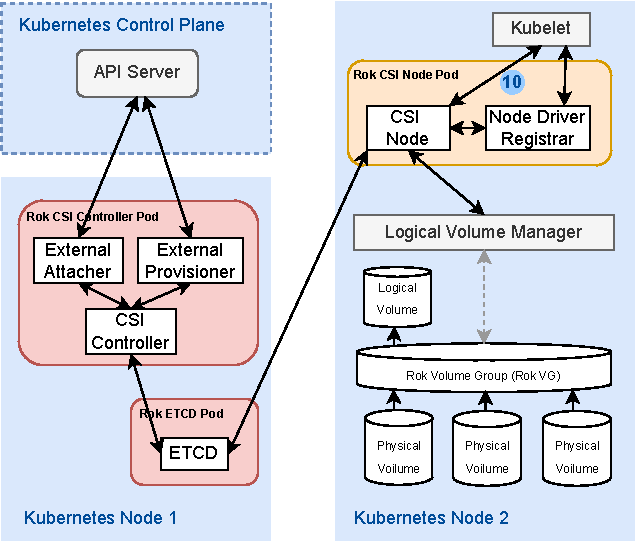
\includegraphics[width=0.9\textwidth]{resources/rok-csi-architecture.pdf}
      \caption{Η αρχιτεκτονική του συστήματος αποθήκευσης του Rok}
      \label{figure:gr-rok-csi-architecture}
\end{figure}
